\chapter{Successioni e serie di funzioni}
Il capitolo tratterà lo studio di successioni e serie di funzioni. I due argomenti sono tra loro collegati. Tuttavia, sebbene si possa ricondurre lo studio di una serie a quello di una successione, la successione delle ridotte n-esime, il capitolo non le porterà avanti in parallelo ma le analizzerà una per volta.
\section{Successioni di funzioni}
\begin{definition} \label{Def: Successione di funzioni}
     Si dice \textbf{successione di funzioni} l'insieme $\{\fn\}_{n \in \N}$ con
     \begin{equation}
         \fn: I \subseteq \R \to \R, n \in \N
     \end{equation}
\end{definition}
\begin{oss}
    Per questioni di praticità, laddove sia utilizzata una successione di funzioni, questa verrà indicata con $\fn$ anziché con $\{\fn\}_n\in \N$.
\end{oss}
Definito il concetto di successione di funzioni, si può iniziare a studiare la convergenza nelle sue diverse forme.\\
Si può innanzitutto notare che, fissato $\overline{x}\in I$, 
allora $\{\fn(\overline{x})\}_{n \in \N}$ è una successione numerica.
\begin{definition} \label{Def: Convergenza puntuale succ}
    Sia $\fn$ una successione di funzioni $I\to \R$. Allora si dice che $\fn$ \textbf{converge puntualmente} alla funzione $f: I \to \R$ se per ogni $\overline{x} \in I$ si ha che
    \begin{equation}
        \lim_{n \to +\infty} \fn(\overline{x}) = f(\overline{x})
    \end{equation}
    cioè
    \begin{equation}
        \forall\ \overline{x} \in I,\ \forall\ \varepsilon > 0,\ \exists\ N_{\varepsilon, x} \in \N\ \text{tale che}\ \forall\ n> N_{\varepsilon,x}\ \text{si ha}\ \left| \fn(x)-f(x)\right| < \varepsilon
    \end{equation}
    o, equivalentemente, sfruttando il criterio di Cauchy puntuale, se
\begin{equation}
    \forall\ x \in I, \forall\ \varepsilon > 0\ \exists\ N_{\varepsilon, x} \in N\ \text{tale che}\ \forall\ n,m > N_{\varepsilon, x}\ \text{si ha che}\ |\fn - f_m|<\varepsilon
\end{equation}
\end{definition}    
\begin{definition} \label{Def: Funzione limite}
    Inoltre, se c'è convergenza puntuale in $I$, è ben definita la \textbf{funzione limite} $f: I \to \R$ tale che
    \begin{equation}
        f(x) := \lim_{n \to +\infty} \fn(x)
    \end{equation}
\end{definition}
Occorre osservare che nel caso della convergenza puntuale, $N$ dipende e da $\varepsilon$ e da $x$, pertanto può essere utile dare una definizione più forte di convergenza che non dipenda da $x$.
\begin{definition} \label{Def: Convergenza uniforme succ}
    Si dice che $\fn$ \textbf{converge uniformemente} su $I$ a $f: I \to \R$ se
    \begin{equation}
        \forall\ \varepsilon>0\ \exists\ N_\varepsilon \in \N\ \text{tale che}\ \forall\ n>N_\varepsilon\ \text{si ha}\ \sup_{x \in I}|\fn(x)-f(x)| < \varepsilon
    \end{equation}
    cioè se
    \begin{equation}
    \lim_{n \to + \infty}{\sup_{x \in I} \left| \fn(x)-f(x)\right|}=0
    \end{equation}
    o, tramite il criterio di Cauchy uniforme,
    \begin{equation}
        \forall \ \varepsilon >0 \ \exists\ N_\varepsilon \in \N \ \text{tale che}\ \forall\ n,m > N_\varepsilon\ \text{si ha}\ \sup_{x \in I}{|\fn(x)-f_m(x)|}<\varepsilon
    \end{equation}
\end{definition}
\begin{figure}[H]
    Graficamente, la convergenza uniforme fa sì che si verifichi una situazione di questo tipo.
    \centering
        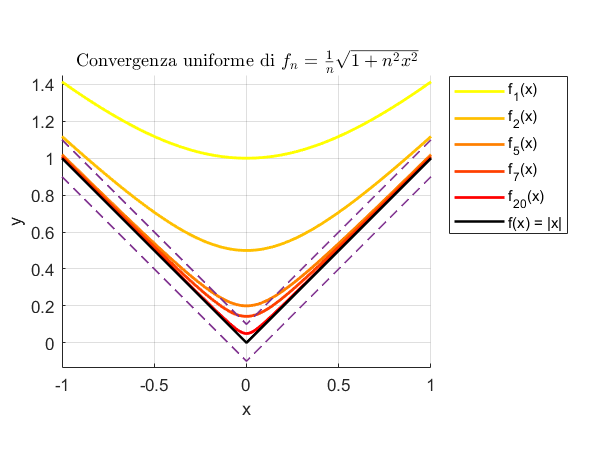
\includegraphics[width=0.4\textwidth]{Capitoli/Capitolo7/Convergenza uniforme.png}
\end{figure}
\begin{oss}
   Si può notare che la convergenza uniforme implica la convergenza puntuale, ma non è necessariamente vero il contrario.
    \end{oss}
\begin{oss}
 Dal punto di vista operativo, per stabilire l'uniforme convergenza di una successione di funzioni, si può agire in due modi:
    \begin{itemize}
       \item Calcolare $\sup\limits_{x \in I} |\fn(x)-f(x)|$ ricercando massimi e minimi con gli strumenti del calcolo in una variabile.
       \item Maggiorare opportunamente $\sup\limits_{x \in I} |\fn(x)-f(x)|$.
\end{itemize}
\end{oss}
\begin{example}
Si studi ora la convergenza della seguente successione di funzioni, il cui grafico è riportato in figura
\begin{equation*}
    \fn= x^n, \qquad x \in [0,1]
\end{equation*}
\begin{figure}[H]
    \centering
\begin{minipage}{0.6\textwidth}
Per quanto riguarda la convergenza puntuale si osserva che, fissato $x \in [0,1]$,
\begin{equation*}
    \lim_{n \to +\infty}{\fn(x)}= \lim_{n \to + \infty}= f(x) = \begin{cases}
        0 &\quad x \in [0,1]\\
        1 &\quad x=1
    \end{cases}
\end{equation*}
\end{minipage}
    \begin{minipage}{0.38\textwidth}
        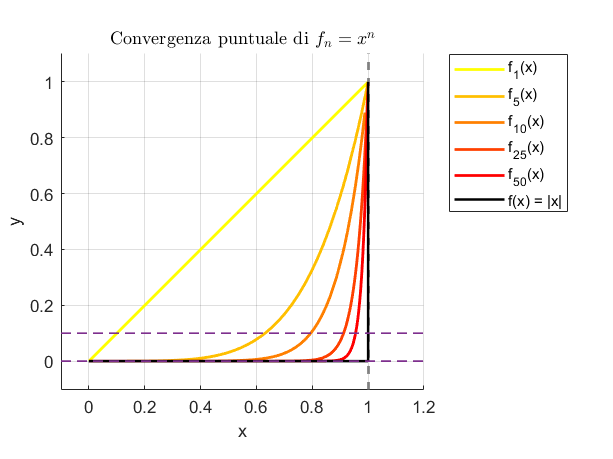
\includegraphics[width=\textwidth]{Capitoli/Capitolo7/Convergenza puntuale.png}
    \end{minipage}
    \end{figure}
Volendo poi studiare la convergenza uniforme, si ha che
\begin{equation*}
    \sup_{x \in [0,1]}{\left|\fn(x)-f(x)\right|} = \sup_{x \in [0,1]} \left\{ \sup_{x \in [0,1)} \left|\fn(x)-f(x)\right|, \left|\fn(x)-f(x)\right|\right\} = \sup_{x \in [0,1)}{\left|x^n-0\right|} = 1 \neq 0
\end{equation*}
Dunque in $[0,1]$ $\fn$ non converge in modo uniforme. D'altra parte è anche vero che la "patologia" si verifica in $x=1$, perciò valutando la convergenza uniforme in $[0,a],\ a < 1$, si ha che
\begin{equation*}
    \sup_{x \in [0,a]}{|\fn(x)-f(x)|}= x^n \big|_{[0,a]} = a^n \overset{n \to +\infty}{\to} 0
\end{equation*}
cioè $\fn$ uniformemente convergente a $0$ su ogni compatto $[0,a],\ a<1$.
\end{example}
\begin{theorem}[Scambio di limiti] \label{Teo: Scambio di limiti}
Sia $\fn: I \to \R$ tale che $\{\fn\}_n$ converge uniformemente in $I$ a $f: I \to \R$. Sia $x_0$ un punto di accumulazione per $I$ e si supponga che per ogni $n \in \N$ esista
\begin{equation}
    \ell_n:= \lim_{x \to x_0}{\fn(x)} \in \R
\end{equation}
Allora esistono i seguenti limiti e si ha
\begin{equation}
    \lim_{n \to +\infty}{\left(\lim_{x \to x_0} {\fn(x)}\right)}= \lim_{n \to +\infty}{\ell_n} = \lim_{x \to x_0} {f(x)} = \lim_{x \to x_0}{ \left( \lim_{n \to +\infty} {\fn(x)}\right)}
\end{equation}
\end{theorem}
\begin{proof}
    Si mostri che $\ell_n$ è una successione di Cauchy.\\
    Dalla convergenza uniforme delle $f_n$ si ha che
    \begin{equation}
        \forall\ \varepsilon>0\ \exists\ N_\varepsilon \in \N\ \text{tale che}\ \left| \fn(x)-f(x)\right|< \varepsilon,\ \forall\ x \in I
    \end{equation}
    Perciò, passando al limite per $x \to x_0$, si ha che
    \begin{equation}
        \left| \lim_{x \to x_0}{\fn(x)}-\lim_{x \to x_0}{f(x)}\right| = \left| \ell_n - \ell_m \right| \leq \varepsilon
    \end{equation}
    cioè $\ell_n$ è di Cauchy. Inoltre, $\{\ell_n\}_n$ è una successione di numeri reali, dunque essa deve convergere ad un qualche $\ell \in \R$. Ciò dimostra la prima metà della tesi.\\
    Rimane da provare che $f(x) \overset{x \to x_0}{\to} \ell$, cioè che $|f(x)-\ell| \to 0$. Dunque,
    \begin{equation}
    \begin{aligned}
        \left|f(x)-\ell\right| &= \left| f(x) - f_\nu(x)+ f_nu(x)- \ell_nu+ \ell_nu- \ell\right| =\\
        &=\overset{\text{Triang.}}{\leq} \left| f(x) - f_\nu(x) \right| +\left| f_\nu(x)- \ell_\nu(x)\right|+\left|\ell_\nu-\ell\right|
    \end{aligned}
    \end{equation}
    Si può notare che il primo termine è minore di $\varepsilon$ per ogni $\nu > N_\varepsilon$ per convergenza uniforme e che il terzo, essendo una successione numerica, è minore di $\varepsilon$ per un $\nu$ sufficientemente grande, poiché $\ell_n \to \ell$. Il secondo, fissato $\nu$ come sopra, soddisfa per ipotesi
    \begin{equation}
        \lim_{x \to x_0}{f_\nu(x)} = \ell_\nu
    \end{equation}
    Dunque, esiste un intorno $\U(x_0)$ tale che per ogni $ \in \U(x_0)$, $\left| f_\nu(x)- \ell_nu \right| < \varepsilon$.\\
    In conclusione, per $\nu$ fissato come sopra e $x \in \U(x_0)$ si ha che
    \begin{equation}
        \left|f(x)-\ell\right| < 3 \varepsilon
    \end{equation}
\end{proof}
\begin{oss}
    Il passaggio al limite nella prima parte della dimostrazione è consentito dal fatto che per ipotesi siano definite $\ell_n$ e $\ell_m$ reali.
\end{oss}
Da tale teorema discende come conseguenza immediata il seguente corollario
\begin{corollary}
    Sia $\fn$ una successione di funzioni continue uniformemente convergente in $I$ a $f:I \to \R$. Allora $f$ è continua. 
\end{corollary}
\begin{proof}
    Si mostri che preso $x_0$ punto di accumulazione per $I$, si ha
    \begin{equation}
        \lim_{x \to x_0}{f(x)}= f(x_0)
    \end{equation}
    Dunque sfruttando l'ipotesi di convergenza, si ha che
    \begin{equation}
        \lim_{x \to x_0}{\fn(x)}= \fn(x_0) \in \R
    \end{equation}
    D'altra parte vale lo scambio di limiti, quindi
    \begin{equation}
    \begin{aligned}
          f(x_0) &=  \lim_{n \to +\infty}{\fn(x_0)}= \lim_{n \to +\infty}{\left(\lim_{x \to x_0}{\fn(x)}\right)}=\\
          &= \lim_{x \to x_0}{ \left( \lim_{n \to +\infty}{\fn(x)}\right)}=\lim_{x \to x_0}{f(x)} 
    \end{aligned}
    \end{equation}
   
\end{proof}
Si mostrino ora due importanti risultati rispetto alla derivazione e all'integrazione di successioni di funzioni.
\begin{theorem} \label{Teo: Passaggio al limite sotto al segno di derivata}
    Sia $\{\fn\}_{n\in\N}$ una successione di funzioni $C^1[a,b]$. Sia la successione di numeri reali $\{\fn(x_0)\}_n$ convergente e sia $\{\fn'\}_n$ uniformemente convergente. Allora $\{\fn\}_n$ converge uniformemente in $[a,b]$ ad una funzione $f \in C^1([a,b])$ e 
    \begin{equation}
        \lim_{n \to +\infty}{\fn'(x)}= \left(\lim_{n \to +\infty}{\fn(x)}\right)'=f'(x)
    \end{equation}
\end{theorem}
\begin{theorem} \label{Teo: Passaggio al limite sotto al segno di integrale}
Sia $\{\fn\}_{n_\in \N}$ una successione di funzioni continue in $[a,b]$ uniformemente convergente in $[a,b]$ a $f$. Allora
\begin{equation}
    \lim_{n \to +\infty}{\int\limits_{a}^{b}{\fn(x)}\,dx}=\int\limits_{a}^{b}{\lim_{n \to +\infty}{\fn(x)}\,dx}= \int\limits_{a}^{b}{f(x)}\,dx
\end{equation}
\end{theorem}
\begin{example}
    In questo esempio si può osservare quanto sia rilevante l'ipotesi di uniforme convergenza della successione.
    \begin{figure}[H]
        \centering
        \begin{minipage}{0.5\textwidth}
            Si consideri la successione di funzioni data da 
            \begin{equation*}
            f_n(x)=\begin{cases}
            0 &\qquad x=0\\
            n & \qquad x \in (0, \frac{1}{n})\\
            0 &\qquad x \in (\frac{1}{n}, 1)\\
            \end{cases}
            \end{equation*}
            e si osservi che
            \begin{equation*}
                \int\limits_{0}^{1}{\fn(x)}\,dx=1 \neq \int\limits_{0}^{1}{f(x)}\,dx = 0
            \end{equation*}
        \end{minipage}
        \begin{minipage}{0.4\textwidth}
        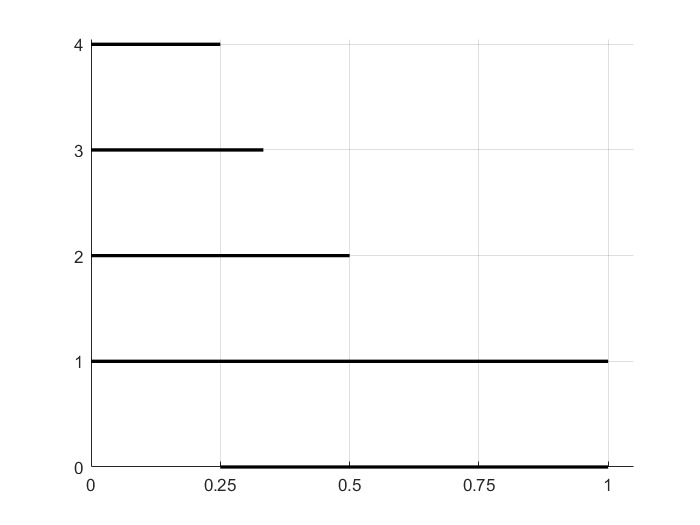
\includegraphics[width=\textwidth]{Capitoli/Capitolo7/Esempio integrale succ. funz..png}
        \end{minipage}
    \end{figure}
    poiché non uniformemente convergente.
\end{example}
\section{Serie di funzioni}
Come già accennato all'inizio del capitolo, quando si parla di serie, ci si può in realtà rifare alle successioni. Perciò in questa sezione verranno rielaborate le informazioni del capitolo precedente adattandole alle serie di funzioni.
\begin{definition}
    Sia $\{\fn\}_{n \in \N}$ una successione di funzioni, $\fn: I \subseteq \R \to \R$. Si dice \textbf{serie di funzioni} di termine generale $\fn$ la successione di funzioni delle somme parziali di $\{\fn\}_{n \in \N}$ data da
    \begin{equation}
        \sn(x)=\sum\limits_{n=1}^{N}{\fn(x)}
    \end{equation}
\end{definition}
Si passi alla convergenza.
\begin{definition}
    Sia $\{\sn\}_{n \in \N}$ una serie di funzioni. Allora si dice che la serie \textbf{converge puntualmente} in I se la successione $\{\sn\}_{n \in \N}$ converge puntualmente in I. In maniera equivalente, la serie converge se, detta
    \begin{equation}
        s(x)=\lim_{n \to +\infty}{\sn(x)}
    \end{equation}
    si ha che
    \begin{equation}
        \forall\ x \in I,\ \forall\ \varepsilon>0,\ \exists\ N_{\varepsilon, x}\ \text{tale che}\ \forall N>N_{\varepsilon, x}\ \text{si ha che}\ |\sn(x)-s(x)|< \varepsilon
    \end{equation}
    o, ancora, sfruttando il criterio di Cauchy, se
    \begin{equation}
        \forall\ x \in I,\ \forall\ \varepsilon>0,\ \exists\ N_{\varepsilon, x}\ \text{tale che}\ \forall\ n>N_{\varepsilon, x},\ \forall p \in \N\ \text{si ha}\ |f_{n+1}(x)+ \dots+ f_{n+p}(x)|<\varepsilon
    \end{equation}
\end{definition}
\begin{definition}
    Se la serie converge puntualmente è ben definita la funzione \textbf{somma}
    \begin{equation}
        s(x)=\lim_{n \to +\infty}{\sn(x)}= \sum_{n=0}^{\infty}{\fn(x)}
    \end{equation}
\end{definition}
\begin{definition}
Sia $\{\sn\}_{n \in \N}$ una serie di funzioni. Allora si dice che la serie \textbf{converge uniformemente} in I se la successione $\{\sn\}_{n \in \N}$ converge uniformemente in I. In maniera equivalente, sfruttando il criterio di Cauchy uniforme, se
\begin{equation}
\forall\ \varepsilon>0\ \exists\ N_\varepsilon \in \N\ \text{tale che}\ \forall\ n > N_\varepsilon\ \forall\ p \in \N\ \text{si ha}\ \sup_{x \in I}{|f_{n+1}(x)+\dots+f_{n+p}|}<\varepsilon 
\end{equation}
\end{definition}
%\section{Serie di potenze}
%\section{Spazi metrici}